I figur \ref{fig:q2} the four RMS error for \alpha in the interval from
1 til 200 i displayet. As the figur indekeads the test data, have the
lowest error, and the firste model have the best results. The best value
for \alpha i one, sine the error get biggger the larger \alpha.

\begin{figure}[!htbp]
  \centering
  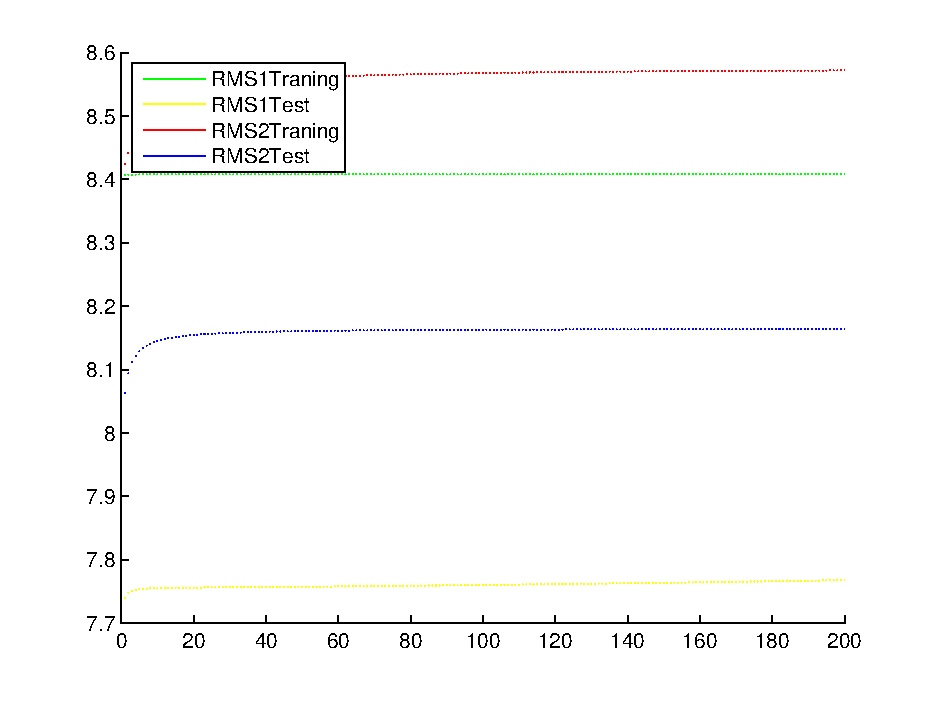
\includegraphics[width=0.6\textwidth]{./images/Q2.pdf}
  \caption{RMS for the 2 traning models and test models}
  \label{fig:q2}
\end{figure}

